\section{Results}
\label{sec:results}

All 1{,}680 model runs (21 datasets $\times$ 10 folds $\times$ 8 models) completed without failure. The analyses below
follow the written analysis plan (Section~\ref{sec:design}); the statistics were recomputed from the raw per-fold results by a second, separately written
implementation (exact Wilcoxon enumeration, hand-coded Friedman and Holm procedures) with identical results. Both
implementations were written with the same AI assistant (see the note on page 1), so this check guards against
coding errors, not against a shared misunderstanding.

\subsection{Classification}
On the primary metric, log loss, Kumo Tabular had the best average rank among the eight models (1.07; Friedman
$p<0.001$; Table~\ref{tab:ranks}, Figure~\ref{fig:ranks}). It had a lower log loss than CatBoost, random forests,
extra trees, histogram gradient boosting, XGBoost and LightGBM on all 15 datasets, and than logistic regression on 14 of
15 (Table~\ref{tab:comparison}). All seven differences remain significant after Holm's correction (adjusted $p<0.001$).
The median relative reduction in log loss ranged from 12.8\% against CatBoost to 54.5\% against extra trees. Against the
strongest baseline on each individual dataset, Kumo Tabular had the lower log loss on 14 of 15 datasets; on
\texttt{climate-model-simulation-crashes} logistic regression was marginally better (0.1311 versus 0.1313;
Figure~\ref{fig:perdataset}).

Because log loss rewards calibrated probabilities, and tree ensembles are often poorly calibrated, a log-loss advantage
could reflect calibration alone. The secondary metrics speak against this explanation. Kumo Tabular also had the best
average rank for one-vs-rest ROC-AUC (1.33), which depends only on the ordering of predictions, and for accuracy (1.77)
and macro-F1 (2.20). These secondary comparisons are descriptive, but each of the seven pairwise comparisons on each
secondary metric favoured Kumo Tabular on at least 11 of 15 datasets. Its advantage in accuracy is not uniform: relative
to the best baseline on each dataset it was lower on \texttt{diabetes} ($-1.8$ percentage points),
\texttt{climate-model-simulation-crashes} ($-1.1$) and \texttt{kc2} ($-0.2$), equal on \texttt{pc3}, and largest on
\texttt{vehicle} ($+11.5$) and \texttt{balance-scale} ($+10.4$).

\begin{table}[t]
\centering
\small
\caption{Kumo Tabular versus each baseline on the primary metric, with datasets as the unit of analysis. W/T/L: datasets on which Kumo is better/equal/worse. Relative advantage: median over datasets of the baseline's loss minus Kumo's loss, divided by the baseline's loss (positive favours Kumo). $p$: two-sided Wilcoxon signed-rank test; Holm: adjusted across the seven baselines of a task. Avg.\ rank: average rank among all eight models (1 = best).}
\label{tab:comparison}
\begin{tabular}{llcrrrr}
\toprule
Task (metric) & Baseline & W/T/L & Rel.\ adv. & $p$ & Holm $p$ & Avg.\ rank \\
\midrule
\multirow{8}{*}{\shortstack[l]{Classification (log loss)\\$n=15$}} & Kumo Tabular & -- & -- & -- & -- & 1.07 \\
& CatBoost & 15/0/0 & +12.8\% & $<$0.001 & $<$0.001 & 2.47 \\
& Logistic reg. & 14/0/1 & +20.5\% & $<$0.001 & $<$0.001 & 3.73 \\
& Random forest & 15/0/0 & +40.2\% & $<$0.001 & $<$0.001 & 5.00 \\
& XGBoost & 15/0/0 & +33.0\% & $<$0.001 & $<$0.001 & 5.07 \\
& Extra trees & 15/0/0 & +54.5\% & $<$0.001 & $<$0.001 & 6.00 \\
& HistGB & 15/0/0 & +42.8\% & $<$0.001 & $<$0.001 & 6.33 \\
& LightGBM & 15/0/0 & +40.8\% & $<$0.001 & $<$0.001 & 6.33 \\
\midrule
\multirow{8}{*}{\shortstack[l]{Regression (RMSE)\\$n=6$}} & Kumo Tabular & -- & -- & -- & -- & 1.67 \\
& CatBoost & 5/0/1 & +2.7\% & 0.156 & 0.312 & 2.67 \\
& Extra trees & 5/0/1 & +10.4\% & 0.094 & 0.281 & 3.50 \\
& XGBoost & 5/0/1 & +12.8\% & 0.156 & 0.312 & 4.17 \\
& Random forest & 5/0/1 & +9.6\% & 0.062 & 0.250 & 4.33 \\
& HistGB & 6/0/0 & +15.8\% & 0.031 & 0.219 & 5.33 \\
& LightGBM & 6/0/0 & +15.9\% & 0.031 & 0.219 & 6.33 \\
& Linear reg. & 6/0/0 & +48.7\% & 0.031 & 0.219 & 8.00 \\
\bottomrule
\end{tabular}
\end{table}


\begin{table}[t]
\centering
\small
\caption{Average rank of each model per metric (1 = best) and Friedman test $p$-value. Primary metrics in the first column of each task; the others are descriptive.}
\label{tab:ranks}
\begin{tabular}{lcccc|ccc}
\toprule
& \multicolumn{4}{c|}{Classification ($n=15$)} & \multicolumn{3}{c}{Regression ($n=6$)} \\
Model & log loss & accuracy & ROC-AUC & macro-F1 & RMSE & MAE & $R^2$ \\
\midrule
Kumo Tabular & 1.07 & 1.77 & 1.33 & 2.20 & 1.67 & 1.33 & 1.67 \\
Logistic reg. & 3.73 & 3.93 & 4.40 & 4.80 & -- & -- & -- \\
Linear reg. & -- & -- & -- & -- & 8.00 & 8.00 & 8.00 \\
Random forest & 5.00 & 6.20 & 5.27 & 6.07 & 4.33 & 4.67 & 4.33 \\
Extra trees & 6.00 & 5.27 & 5.60 & 5.80 & 3.50 & 3.17 & 3.50 \\
HistGB & 6.33 & 5.23 & 5.40 & 4.60 & 5.33 & 5.67 & 5.50 \\
XGBoost & 5.07 & 4.60 & 5.13 & 3.73 & 4.17 & 3.67 & 4.33 \\
LightGBM & 6.33 & 5.23 & 5.93 & 4.60 & 6.33 & 6.67 & 6.17 \\
CatBoost & 2.47 & 3.77 & 2.93 & 4.20 & 2.67 & 2.83 & 2.50 \\
\midrule
Friedman $p$ & $<$0.001 & $<$0.001 & $<$0.001 & $<$0.001 & $<$0.001 & $<$0.001 & $<$0.001 \\
\bottomrule
\end{tabular}
\end{table}


\begin{figure}[t]
\centering
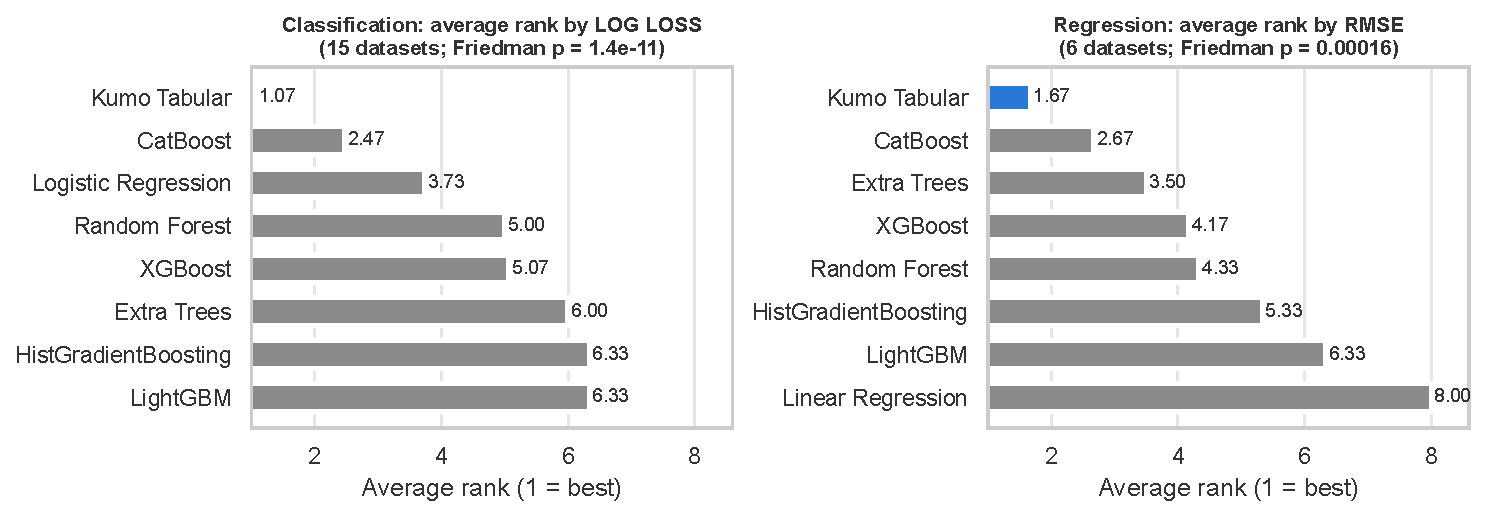
\includegraphics[width=\textwidth]{figures/average_ranks.pdf}
\caption{Average rank of each model on the primary metric across datasets (1 = best). Kumo Tabular in blue.}
\label{fig:ranks}
\end{figure}

\subsection{Regression}
On RMSE, Kumo Tabular had the best average rank (1.67; Friedman $p<0.001$), followed by CatBoost (2.67) and extra
trees (3.50); ordinary least squares ranked last on every dataset. Kumo Tabular had a lower RMSE than histogram gradient
boosting, LightGBM and least squares on all six datasets and than the other four baselines on five of six. None of these
differences is significant after Holm's correction (smallest adjusted $p=0.22$), as anticipated by the design: with six
datasets these comparisons cannot reach significance, and we treat them as descriptive. Relative to the best baseline on
each dataset, Kumo Tabular had a lower RMSE on four of six datasets, with the largest reduction on
\texttt{airfoil\_self\_noise} (44\%). It was clearly worse on \texttt{energy\_efficiency}, where its RMSE was 44\% higher
than XGBoost's, and slightly worse on \texttt{red\_wine} (5\% higher than extra trees). The secondary metrics MAE and
$R^2$ gave the same ordering of Kumo Tabular first (average ranks 1.33 and 1.67).

\begin{figure}[t]
\centering
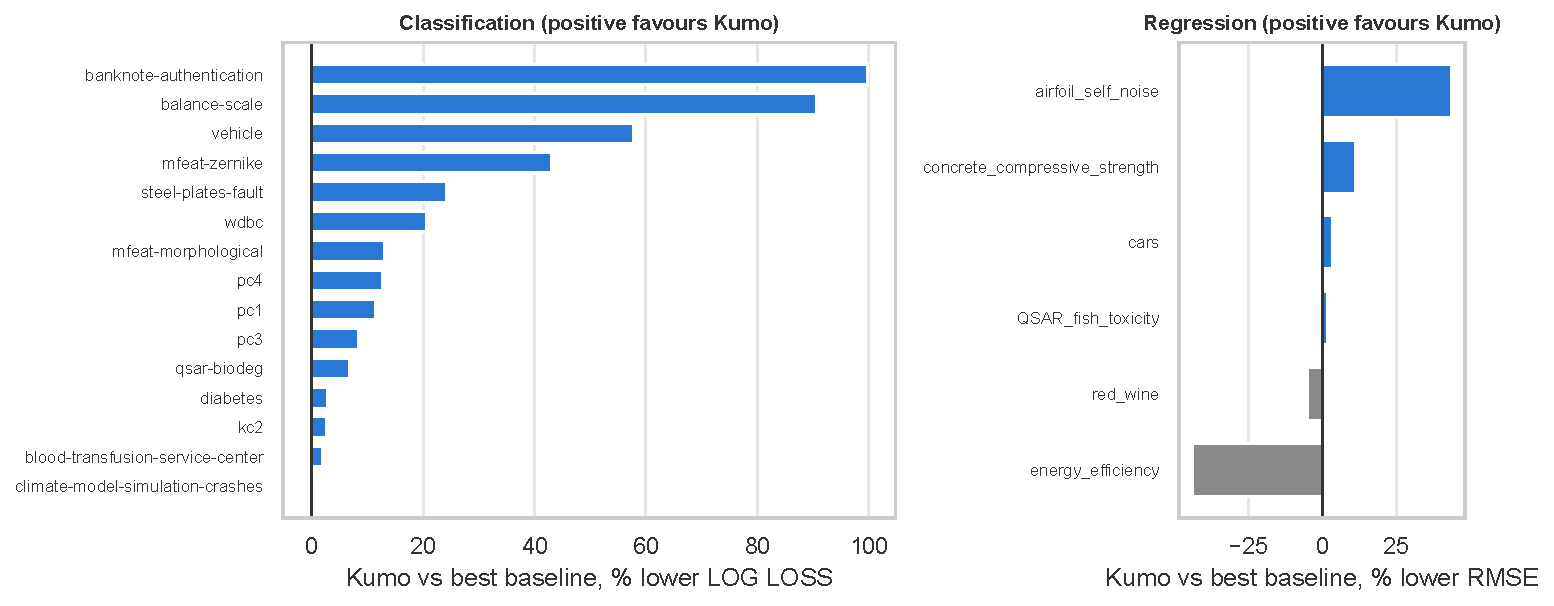
\includegraphics[width=\textwidth]{figures/per_dataset_primary_metric.pdf}
\caption{Per-dataset difference between Kumo Tabular and the best of the seven baselines on that dataset, as a
percentage of the baseline's loss (log loss for classification, RMSE for regression). Positive values favour Kumo
Tabular. Comparing against the per-dataset best baseline is stricter than any single fixed baseline.}
\label{fig:perdataset}
\end{figure}

\subsection{Sensitivity analyses}
The classification conclusions did not change in either planned sensitivity analysis (Table~\ref{tab:sensitivity}).
Without \texttt{wdbc}, Kumo Tabular's average rank was 1.07 and it was significantly better than all seven baselines
after Holm's correction; with related datasets averaged into single units (11 units), its average rank was 1.09 and all
seven comparisons remained significant (adjusted $p=0.007$). The regression results were unchanged because no
regression dataset was affected.

\begin{table}[t]
\centering
\small
\caption{Planned sensitivity analyses on the primary metric: Kumo Tabular's average rank, the number of baselines it beats with Holm-adjusted $p<0.05$, and its W/T/L against the strongest baseline (lowest average rank).}
\label{tab:sensitivity}
\begin{tabular}{llcccc}
\toprule
Task & Analysis & $n$ & Kumo avg.\ rank & Sig.\ wins (of 7) & W/T/L vs strongest \\
\midrule
Classification & All datasets & 15 & 1.07 & 7 & 15/0/0 (CatBoost) \\
 & Excluding wdbc & 14 & 1.07 & 7 & 14/0/0 (CatBoost) \\
 & Families collapsed & 11 & 1.09 & 7 & 11/0/0 (CatBoost) \\
\midrule
Regression & All datasets & 6 & 1.67 & 0 & 5/0/1 (CatBoost) \\
 & Excluding wdbc & 6 & 1.67 & 0 & 5/0/1 (CatBoost) \\
 & Families collapsed & 6 & 1.67 & 0 & 5/0/1 (CatBoost) \\
\bottomrule
\end{tabular}
\end{table}


\subsection{Runtime}
Table~\ref{tab:runtime} and Figure~\ref{fig:runtime} report fit-plus-prediction time per fold. On this hardware the
median time per fold of Kumo Tabular on the GPU (1.27\,s for classification, 1.14\,s for regression) was comparable to
500-tree random forests and extra trees on the CPU and lower than CatBoost with its default 1{,}000 iterations. It was
about 7 (classification) and 9 to 11 (regression) times the median time of XGBoost and LightGBM, and about 48 times
that of logistic regression and 300 times that of least squares. The time per fold depended strongly on
the dataset: on the 10-class \texttt{mfeat-zernike} dataset the ten folds took 1{,}113\,s for histogram gradient
boosting, 841\,s for CatBoost and 650\,s for Kumo Tabular, against 21\,s or less for XGBoost, LightGBM, extra trees and
logistic regression. These measurements are hardware-specific (Section~\ref{sec:limitations}).

\begin{table}[t]
\centering
\small
\caption{Fit plus prediction time per fold in seconds: median [interquartile range] over all folds of all datasets. Kumo Tabular ran on an NVIDIA GTX 980M GPU (float32); all other models on an Intel Core i7-6700HQ CPU. Times are hardware-dependent and not comparable as algorithmic costs.}
\label{tab:runtime}
\begin{tabular}{lll}
\toprule
Model & Classification & Regression \\
\midrule
Kumo Tabular & 1.275 [0.896, 3.053] & 1.142 [0.929, 1.471] \\
Logistic reg. & 0.027 [0.015, 0.053] & -- \\
Linear reg. & -- & 0.004 [0.003, 0.005] \\
Random forest & 1.392 [1.284, 1.542] & 1.077 [1.038, 1.165] \\
Extra trees & 1.087 [1.001, 1.242] & 0.753 [0.737, 0.789] \\
HistGB & 0.487 [0.323, 1.474] & 0.379 [0.341, 0.403] \\
XGBoost & 0.181 [0.114, 0.283] & 0.125 [0.110, 0.152] \\
LightGBM & 0.168 [0.094, 0.318] & 0.103 [0.092, 0.117] \\
CatBoost & 4.564 [3.251, 5.824] & 1.728 [1.348, 2.018] \\
\bottomrule
\end{tabular}
\end{table}


\begin{figure}[t]
\centering
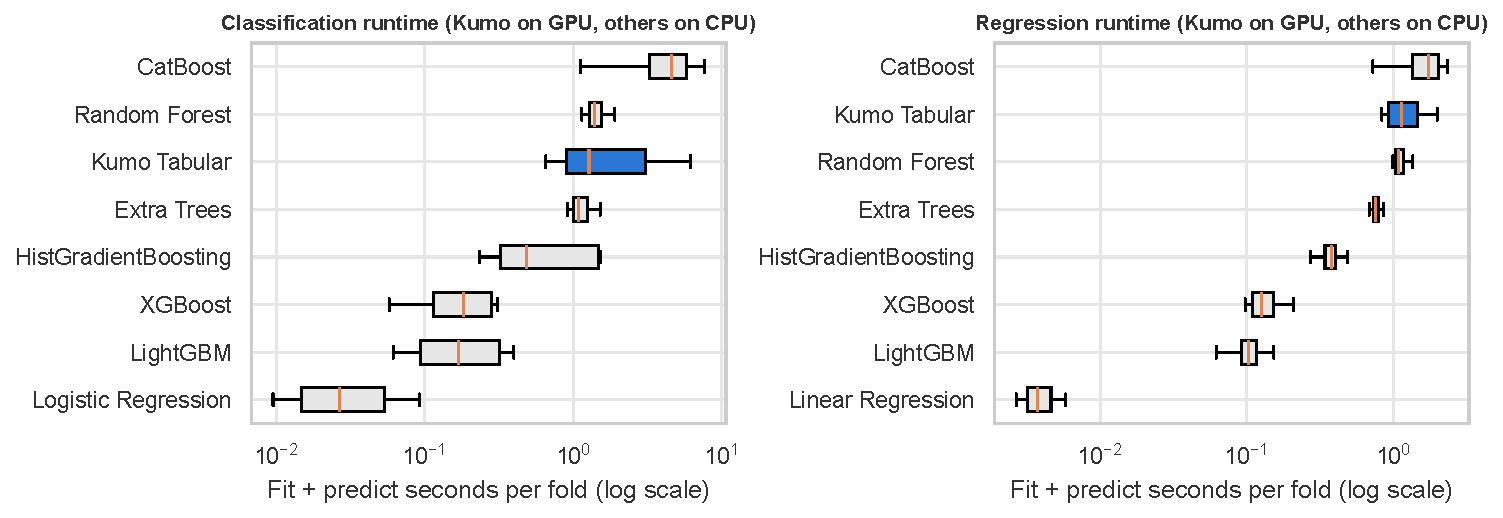
\includegraphics[width=\textwidth]{figures/runtime.pdf}
\caption{Fit plus prediction time per fold (log scale) over all folds of all datasets. Kumo Tabular ran on a GPU, the
other models on a CPU.}
\label{fig:runtime}
\end{figure}

\subsection{Case studies}
\label{sec:case}
The two-dataset case studies (Appendix~\ref{app:case}) are consistent with the benchmark but add detail. On breast
cancer data Kumo Tabular had the best mean on every threshold metric (accuracy 0.989 versus 0.977 for logistic
regression) and higher accuracy than logistic regression on all five splits, but after the overlap correction and Holm's
adjustment no within-dataset comparison was significant (smallest adjusted $p=0.081$). On diabetes data it was
indistinguishable from linear regression ($R^2$ 0.503 versus 0.496). In the training-size study it was much more robust
than least squares with 25 training rows ($R^2$ 0.429 versus 0.075) but no better than logistic regression for
classification at 25 to 100 rows. Its nominal 90\% quantile interval covered 93.3\% of diabetes test targets.
